% \setchapterimage[6cm]{cubism}
% \setchapterpreamble[u]{\begingroup \marginnote[-48mm]{{\begin{flushright} \textcolor{white}{Robert Delaunay,\\ \textit{La fenêtre sur la ville n°3}} \end{flushright}}} \endgroup \margintoc}
\setchapterpreamble[u]{\margintoc}
\chapter{A Model in Cubical Presheaves}
\labch{cubical_model}

As we explained in \cref{sec:univalence}, the central piece of Homotopy Type 
Theory is the univalence axiom, which identifies the type of equalities between 
two types \( A \) and \( B \) with the type of isomorphisms between \( A \) and 
\( B \).
% 
% \[
% (A =_{\varType} B) \enskip \simeq \enskip  (A \simeq B)
% \]

But postulating univalence as an axiom has the unfortunate consequence of 
breaking some of the nice computational properties of intensional type theory.
% 
This is all the more disappointing insofar as the univalence principle has 
constructive models, as evidenced by Bezem \etal who built a model of 
univalence by interpreting types as 
\emph{fibrant cubical sets}~\sidecite{BezemCoquandHuber14}.

This conundrum was solved by the introduction of cubical type 
theories~\sidecite{CCHM,ABCFHL}, which provide an axiom-free univalent system by 
reifying some of the structure of the fibrant cubical sets as syntactical 
constructions.
% 
In this chapter, our aim is to give an alternative solution for computing with
fibrant cubical sets, by presenting the cubical model of Cohen \etal \cite{CCHM} 
as a syntactic translation from \( \MLTT{+}\mathsf{Univalence} \) to a simpler 
type theory.

Our strategy is based on the prefascist translation of Pédrot, which is a 
syntactic account of the interpretation of type theory in categories
of presheaves.
% 
Since the cubical sets of Cohen \etal are presheaves on the 
\emph{category of de Morgan cubes}, we can use the prefascist translation to obtain a 
model of \MLTT in the category of cubical sets. 
% 
However this is not quite sufficient to validate the univalence axiom.
% 
Indeed, the cubical model of Cohen \etal does not exactly follow the generic
recipe to interpret \MLTT in categories of presheaves: in particular, the
equality is interpreted as the set of \emph{cubical paths}, a construction that 
exploits the specific properties of the category of cubes.
% 
And in order to interpret the elimination principle for the equality, Cohen 
\etal equip their cubical sets with \emph{fibration structures}.

\sideremark{The results presented in this chapter have yet to reach the
same degree of maturity as the rest of this thesis. 
We will be careful to distinguish the parts that have been thoroughly checked
from the parts that are less solid.}
% 
In \cref{sec:cubical_sets}, we explain what are cubical sets and fibration 
structures, and how they relate to spaces and topology. 
% 
Then in \cref{sec:cubical_trans} we sketch an extension of the prefascist 
translation of Pédrot with fibration structures, which should give us enough 
structure to interpret the univalence axiom.
% 
Finally, in \cref{sec:cubical-perspectives} we discuss the theoretical 
consequences of this translation.

\section{Cubical Sets and Fibration Structures}
\label{sec:cubical_sets}

Cubical sets were initially studied by topologists, as a candidate for a 
definition of ``space'' that is suitable to do \emph{homotopy theory}, that is 
to study spaces and maps between spaces up to deformations.

When most mathematicians hear the word space, they tend to think of topological
spaces, \ie sets equipped with a lattice of open subsets. 
% 
But while topological spaces may be very well designed for the needs of 
mathematical analysis, it turns out that they are not quite as suitable for 
the study of deformations. 
% 
We can try to explain this mismatch from the definition of a 
\defnote{homotopy}{A homotopy between two continuous maps \( f, g : X \to Y \) 
is a continuous map \( h : X \times [0 , 1] \to Y \) such that 
\( f(x) = h(x, 0) \) and \( g(x) = h(x, 1) \).} between two continuous maps, 
which gives a central role to the interval \( [0, 1] \) ; but topological 
spaces are so general that they have no reason to interact nicely with \( [0, 1] \),
as witnessed by the inadequacy of path-connectedness for general topological 
spaces.

Thus, it should come as no surprise that homotopy theorists like to restrict their 
attention to a subclass of topological spaces that are more compatible with
the unit interval. 
\sideremark{Topological spaces that can be built by iteratively attaching 
cubical cells of increasing dimension are called CW-complexes. Since we only
mention them as motivation, we will not need a precise definition.} 
More specifically, it is common practice to only consider spaces that can be 
built from (hyper)cubes---cartesian powers of the interval---by gluing them together 
(\cref{fig:cubical-set}). This way, we can be sure that they do not 
get too wild and the definition of homotopy will be reasonable.

\begin{figure}[!h]
    \tikzset{every picture/.style={line width=0.75pt}} %set default line width to 0.75pt        
    
    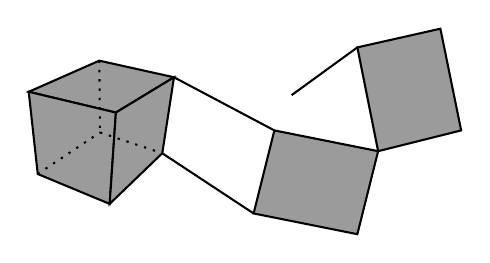
\begin{tikzpicture}[x=0.75pt,y=0.75pt,yscale=-1,xscale=1]
        %uncomment if require: \path (0,300); %set diagram left start at 0, and has height of 300
        
        %Straight Lines [id:da8704585850733273] 
        \draw    (115.65,43.4) -- (164,69) ;
        %Shape: Polygon [id:ds5510985674035307] 
        \draw  [fill={rgb, 255:red, 155; green, 155; blue, 155 }  ,fill opacity=1 ] (79.65,35.4) -- (115.65,43.4) -- (87.65,60.4) -- (45.65,50.4) -- cycle ;
        %Shape: Polygon [id:ds1595471789989844] 
        \draw  [fill={rgb, 255:red, 155; green, 155; blue, 155 }  ,fill opacity=1 ] (45.65,50.4) -- (87.65,60.4) -- (84.65,104.4) -- (50,90) -- cycle ;
        %Shape: Polygon [id:ds840250297463829] 
        \draw  [fill={rgb, 255:red, 155; green, 155; blue, 155 }  ,fill opacity=1 ] (115.65,43.4) -- (110,80) -- (84.65,104.4) -- (87.65,60.4) -- cycle ;
        %Shape: Polygon [id:ds5116965879899652] 
        \draw  [fill={rgb, 255:red, 155; green, 155; blue, 155 }  ,fill opacity=1 ] (214,79) -- (204,119) -- (154,109) -- (164,69) -- cycle ;
        %Straight Lines [id:da5487647430596088] 
        \draw    (110,80) -- (154,109) ;
        %Straight Lines [id:da03867304181467035] 
        \draw    (172.33,52) -- (204,29) ;
        %Straight Lines [id:da2802264452126314] 
        \draw  [dash pattern={on 0.84pt off 2.51pt}]  (79.65,35.4) -- (80,70) ;
        %Straight Lines [id:da3299433481210239] 
        \draw  [dash pattern={on 0.84pt off 2.51pt}]  (50,90) -- (80,70) ;
        %Straight Lines [id:da5344142761550612] 
        \draw  [dash pattern={on 0.84pt off 2.51pt}]  (80,70) -- (110,80) ;
        %Shape: Polygon [id:ds09674056802999687] 
        \draw  [fill={rgb, 255:red, 155; green, 155; blue, 155 }  ,fill opacity=1 ] (204,29) -- (244,20) -- (254,69) -- (214,79) -- cycle ;
        
    \end{tikzpicture}
    \caption{Building a space by gluing cubes of various dimensions together}
    \label{fig:cubical-set}
\end{figure}

Now, this idea of building objects by taking amalgamated sums of a family of
basic ``building block'' objects should be reminiscent of the previous chapter
about presheaves, and the reader might be wondering if we can use 
presheaves on an appropriate category of cubes to obtain a synthetic model of
well-behaved spaces.
% 
This is precisely what cubical sets are.

\subsection{The category of cubes}
\label{sec:cat_cubes}

We now define the category of \defnote{cubes}{By cubes, we mean generalized cubes
of all integer dimensions: the point, the segment, the square, the 3D cube, the 
4D hypercube... are all cubes.} \( \catCube \). Since our building blocks 
are cubes of all integer dimensions (including a cube of dimension zero, which is a 
point), we will have one object per dimension:
\[
    \obj{\catCube} := \Nat.
\]
Thus, the objects of \( \catCube \) are integers, that we shall mentally
picture as cubes of the corresponding dimension:
% 
\begin{figure}[!h]
    \tikzset{every picture/.style={line width=0.75pt}} %set default line width to 0.75pt        
    
    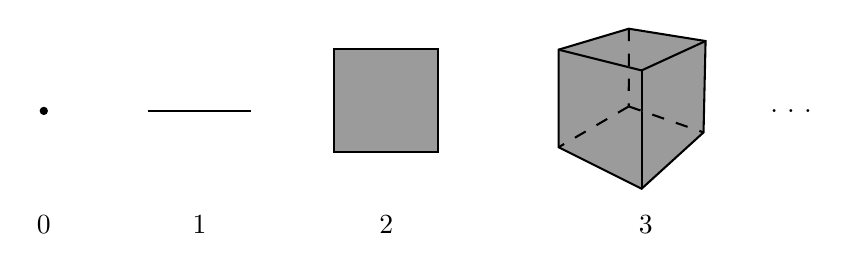
\begin{tikzpicture}[x=0.75pt,y=0.75pt,yscale=-1,xscale=1,roundnode/.style={circle, fill=black, inner sep=0pt, minimum size=0pt}] % 3pt
        %Dimension 0
        \node[circle, fill=black, inner sep=0pt, minimum size=3pt] (A) at (50,70) {};
        \node[] (A5) at (50, 125) {$0$};
        
        %Dimension 1
        %Straight Lines [id:da5345039200266992] 
        \draw    (100,70) -- (150,70) ;
        \node[roundnode] (B0) at (100,70) {};
        \node[roundnode] (B1) at (150,70) {};
        \node[] (B5) at (125, 125) {$1$};

        %Dimension 2
        %Shape: Rectangle [id:dp20722346190864016] 
        \draw  [fill={rgb, 255:red, 155; green, 155; blue, 155 }  ,fill opacity=1 ] (190,40) -- (240,40) -- (240,90) -- (190,90) -- cycle ;
        \node[roundnode] (C00) at (190,40) {};
        \node[roundnode] (C01) at (240,40) {};
        \node[roundnode] (C11) at (240,90) {};
        \node[roundnode] (C10) at (190,90) {};
        \node[] (A5) at (215, 125) {$2$};

        %Dimension 3
        %Shape: Polygon [id:ds3964990966713411] 
        \draw  [fill={rgb, 255:red, 155; green, 155; blue, 155 }  ,fill opacity=1 ] (368.83,36.34) -- (367.85,80.35) -- (338,107.5) -- (298,87.5) -- (298,40.5) -- (331.85,30.4) -- cycle ;
        %Straight Lines [id:da9527006690207834] 
        \draw [fill={rgb, 255:red, 155; green, 155; blue, 155 }  ,fill opacity=1 ]   (298,40.5) -- (338,50.5) ;
        %Straight Lines [id:da7924166842637828] 
        \draw [fill={rgb, 255:red, 155; green, 155; blue, 155 }  ,fill opacity=1 ]   (338,50.5) -- (338,107.5) ;
        %Straight Lines [id:da09670577736593144] 
        \draw [fill={rgb, 255:red, 155; green, 155; blue, 155 }  ,fill opacity=1 ]   (338,50.5) -- (368.83,36.34) ;
        %Straight Lines [id:da9435691747263029] 
        \draw [fill={rgb, 255:red, 155; green, 155; blue, 155 }  ,fill opacity=1 ] [dash pattern={on 4.5pt off 4.5pt}]  (331.83,67.84) -- (298,87.5) ;
        %Straight Lines [id:da6208721194399572] 
        \draw [fill={rgb, 255:red, 155; green, 155; blue, 155 }  ,fill opacity=1 ] [dash pattern={on 4.5pt off 4.5pt}]  (331.83,67.84) -- (367.85,80.35) ;
        %Straight Lines [id:da9613978440337915] 
        \draw [fill={rgb, 255:red, 155; green, 155; blue, 155 }  ,fill opacity=1 ] [dash pattern={on 4.5pt off 4.5pt}]  (331.85,30.4) -- (331.83,67.84) ;
        \node[roundnode] (D000) at (298,40.5) {};
        \node[roundnode] (D001) at (338,107.5) {};
        \node[roundnode] (D011) at (368.83,36.34) {};
        \node[roundnode] (D010) at (298,87.5) {};
        \node[roundnode] (D110) at (367.85,80.35) {};
        \node[roundnode] (D100) at (331.85,30.4) {};
        \node[roundnode] (D111) at (338,50.5) {};
        \node[roundnode] (D101) at (331.83,67.84) {};
        \node[] (A5) at (340, 125) {$3$};

        \node[] (E) at (410,70) {$.\ .\ .$};
    \end{tikzpicture}
    \caption{Graphical representation of the first four objects of \( \catCube \)}
\end{figure}

Then, the set of morphisms \( \hom[\catCube]{m}{n} \) between any two such objects should 
intuitively encode the different ways to send a cube of dimension \( m \) to
a cube of dimension \( n \).
%  
There are many reasonable choices for this definition 
(see \sidecitet{BuchholtzMorehouse17} for a survey), and each choice will 
result in a slightly different category of cubical sets. 
\sideremark{The hope is that these different categories of cubical sets will
capture the same notion of space, when considered up to homotopy. But such
theorems are usually quite difficult to prove.}
% 
In this chapter, we follow Cohen et al. \cite{CCHM} and use the category of 
\emph{de Morgan} cubes:
\begin{definition}\label{def:cat_cubes}
    The category of de Morgan cubes \( \catCube \) is defined by
    \begin{align*}
        & \obj{\catCube} := \Nat \\
        & \hom[\catCube]{m}{n} := \mathrm{Vec}(\demorgan{x_1, ..., x_m}, n),
    \end{align*}
    meaning that the morphisms from \( m \) to \( n \) are lists of \( n \) 
    terms of \( \demorgan{x_1, ..., x_m} \), the free de Morgan algebra on 
    \( m \) variables.
\end{definition}
% 
The definition of a de Morgan algebra is presented in \cref{fig:deMorgan}.

The identity of \( \hom[\catCube]{n}{n} \) is given by listing the variables
in order:
\[
    \mathrm{Id}_n := \langle x_1 , ... , x_n \rangle,
\]
and given two morphisms
\( \langle i_1 , ... , i_m \rangle \in \hom[\catCube]{l}{m} \)
and \( \langle j_1 , ... , j_n \rangle \in \hom[\catCube]{m}{n} \), their 
composition is given by substitution:
\begin{align*}
    & \langle j_1 , ... , j_n \rangle \circ \langle i_1 , ... , i_m \rangle := \\
    & \quad \langle j_1[x_1 \leftarrow i_1, ..., x_m \leftarrow i_m] , ... , j_n[x_1 \leftarrow i_1, ..., x_m \leftarrow i_m] \rangle.
\end{align*}
% 
One readily checks that these definitions satisfy the axioms of a category.
From there, we can define cubical sets as presheaves:
\begin{definition}
    The category of cubical sets is the category of presheaves on de Morgan cubes 
    \( \catCube \).
\end{definition}

\begin{figure}
\begin{small}
    Operations of a de Morgan algebra \( \interval \):
    \[
    \begin{array}{lclcl}
    \izero : \interval & & \land : \interval \times \interval \to \interval & & {\sim} : \interval \to \interval \\
    \ione : \interval & & \lor : \interval \times \interval \to \interval & &
    \end{array}
    \]
    Equations of de Morgan algebras:
    \[
    \begin{array}{cl}
        x \lor (y \lor z) = (x \lor y) \lor z       & \lor-\text{associativity} \\
        \izero \lor x = x = x \lor \izero           & \lor-\text{unit} \\
        \ione \lor x = \ione = x \lor \ione         & \lor-\text{absorption} \\
        x \lor y = y \lor x                         & \lor-\text{symmetry} \\
        x \lor x = x                                & \lor-\text{idempotence} \\
        \hline
        \sim \sim x = x                             & {\sim}-\text{involution} \\
        \sim \izero = \ione                         & {\sim}-\izero \\
        \sim \ione = \izero                         & {\sim}-\ione \\
        \hline
        x \land (y \lor z) = (x \land y) \lor (x \land z) & \text{first distributive law} \\
        x \lor (y \land z) = (x \lor y) \land (x \lor z) & \text{second distributive law} \\
        x = x \lor (x \land y) = x \land (x \lor y) & \text{lattice absorption} \\
        \hline
        {\sim} (x \land y) = {\sim} x \lor {\sim} y & \text{de Morgan's first law} \\
        {\sim} (x \lor y) = {\sim} x \land {\sim} y & \text{de Morgan's second law}
    \end{array}
    \]
\end{small}
    \caption{Definition of a De Morgan algebra}
    \label{fig:deMorgan}
\end{figure}

Now, what is the connection between de Morgan algebras and cubes? First of all,
since cubes are nothing but cartesian powers of the interval (the 
one-dimensional cube), we can expect that the hom-sets of \( \catCube \) are 
entirely determined by the morphisms into the interval. 
\sideremark[*-3]{Recall that \( \hom{A}{B \times C} \cong \hom{A}{B} \times \hom{A}{C} \).}
% 
And while we could have picked \( \hom[\catCube]{n}{1} \) to be the set 
of all real, continuous maps from \( [0, 1]^n \) to \( [0, 1] \), this would result in a 
cumbersome category (we could not expect to have decidable equality on the hom-sets, 
for instance) and it turns out to be unnecessary.
% 
Instead, it will be sufficient for our purposes to only consider a handful of 
primitive continuous maps into the real interval:
\begin{itemize}
    \item cartesian projections \( [0, 1]^n \to [0, 1] \),
    \item constant maps to one of the endpoints of \( [0, 1] \),
    \item \( \min : [0, 1]^2 \to [0, 1] \) and \( \max : [0, 1]^2 \to [0, 1] \), and
    \item \( x \mapsto 1 - x : [0, 1] \to [0, 1] \).
\end{itemize}
% 
And it happens that the hom-sets we obtain after closing this family of
maps under cartesian products and composition are exactly the free de 
Morgan algebras~\sidecite{BuchholtzMorehouse17}.

This restriction seems a bit dramatic: we casually replaced the full set of 
continuous functions with a small set of piecewise linear functions! But the reader
should keep in mind that our goal is to model spaces \emph{up to homotopy},
and we can always deform continuous maps between reasonable spaces into 
piecewise linear maps between cubical spaces~\sidecite{hatcher}.

\subsection{Unfolding definitions}

Now that we defined the category of cubical sets as \( \catPsh{\catCube} \), we
unfold the definition a little bit to get more intuition.
% 
Of course, cubical sets are \emph{combinatorial} objects, meaning that there is 
no topology involved in their definition, but only sets and maps.

A cubical set \( X \) is a functor from \( \op{\catCube} \) to \( \catSet \), 
meaning that we have a set \( X(n) \) for every integer \( n \), representing 
the set of cubes of dimension \( n \) of our cubical set.
% 
Then, the functoriality condition tells us that any map 
\( f : \hom[\catCube]{m}{n} \) in the cube category is sent to a map between 
sets \( X(f) : X(n) \to X(m) \), in a way that respects identities and 
composition. 
% 
We now look at a specific family of basic morphisms that generate all 
morphisms of \( \catCube \), and we analyze their role in cubical sets.
% 
\paragraph{Exchanges and reversals} 
% 
\begin{marginfigure}[*2]

\tikzset{every picture/.style={line width=0.75pt}} %set default line width to 0.75pt        

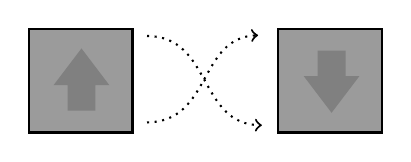
\begin{tikzpicture}[x=0.75pt,y=0.75pt,yscale=-1,xscale=1]
%uncomment if require: \path (0,300); %set diagram left start at 0, and has height of 300

%Shape: Square [id:dp1763700379930293] 
\draw  [fill={rgb, 255:red, 155; green, 155; blue, 155 }  ,fill opacity=1 ] (20,20) -- (70,20) -- (70,70) -- (20,70) -- cycle ;
%Shape: Square [id:dp3508643609243347] 
\draw  [fill={rgb, 255:red, 155; green, 155; blue, 155 }  ,fill opacity=1 ] (140,20) -- (190,20) -- (190,70) -- (140,70) -- cycle ;
%Curve Lines [id:da7064307448895535] 
\draw  [dotted, ->]  (77,23.5) .. controls (108.5,23.67) and (101.5,66.17) .. (132.33,66.5) ;
%Curve Lines [id:da6356525234785018] 
\draw  [dotted, ->]  (77,65.17) .. controls (108.5,64.67) and (101.5,24.17) .. (130.5,23.17) ;
%Right Arrow [id:dp8177216814563346] 
\draw  [draw opacity=0][fill={rgb, 255:red, 128; green, 128; blue, 128 }  ,fill opacity=1 ] (38.71,59.5) -- (38.71,47.17) -- (32,47.17) -- (45.42,29.5) -- (58.83,47.17) -- (52.13,47.17) -- (52.13,59.5) -- cycle ;
%Right Arrow [id:dp30178673917508214] 
\draw  [draw opacity=0][fill={rgb, 255:red, 128; green, 128; blue, 128 }  ,fill opacity=1 ] (172.63,30.5) -- (172.63,42.83) -- (179.33,42.83) -- (165.92,60.5) -- (152.5,42.83) -- (159.21,42.83) -- (159.21,30.5) -- cycle ;

\end{tikzpicture}

\caption{Reversal map}
\label{fig:reversal}

\end{marginfigure}

The \( \sim \) operation of de Morgan algebras gives rise to reversal maps in
the cube category, that mirror \( n \)-dimensional along the \( k \)-th 
dimension for all \( k \le n \):
\[
\mathrm{rev}_k^n := \langle x_1 , ...\ , {\sim} x_k , ...\ , x_n \rangle : \hom[\catCube]{n}{n}
\]
In our cubical set, \( X(\mathrm{rev}_k^n) \) is thus an involution of the set of 
cubes of dimension \( n \), that sends every cube to its ``mirror image'' (which
is simply another element of \( X(n) \)).
Note that the mirror cube will be different from the original, meaning that the 
cubes that constitute cubical sets are in fact \emph{oriented cubes}.

Likewise, since the objects in our cube category are cartesian powers of the 
interval, we have maps that exchange two dimensions \( j \le k \):
\[
\mathrm{exch}_{j,k}^n := \langle x_1 , ...\ , x_k , ...\ , x_j , ...\ , x_n \rangle : \hom[\catCube]{n}{n}
\]
\begin{marginfigure}[*-3]
\tikzset{every picture/.style={line width=0.75pt}} %set default line width to 0.75pt        

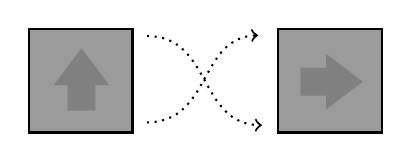
\begin{tikzpicture}[x=0.75pt,y=0.75pt,yscale=-1,xscale=1]
%uncomment if require: \path (0,300); %set diagram left start at 0, and has height of 300

%Shape: Square [id:dp1763700379930293] 
\draw  [fill={rgb, 255:red, 155; green, 155; blue, 155 }  ,fill opacity=1 ] (20,20) -- (70,20) -- (70,70) -- (20,70) -- cycle ;
%Shape: Square [id:dp3508643609243347] 
\draw  [fill={rgb, 255:red, 155; green, 155; blue, 155 }  ,fill opacity=1 ] (140,20) -- (190,20) -- (190,70) -- (140,70) -- cycle ;
%Curve Lines [id:da7064307448895535] 
\draw  [dotted, ->]  (77,23.5) .. controls (108.5,23.67) and (101.5,66.17) .. (132.33,66.5) ;
%Curve Lines [id:da6356525234785018] 
\draw  [dotted, ->] (77,65.17) .. controls (108.5,64.67) and (101.5,24.17) .. (130.5,23.17) ;
%Right Arrow [id:dp8177216814563346] 
\draw  [draw opacity=0][fill={rgb, 255:red, 128; green, 128; blue, 128 }  ,fill opacity=1 ] (38.71,59.5) -- (38.71,47.17) -- (32,47.17) -- (45.42,29.5) -- (58.83,47.17) -- (52.13,47.17) -- (52.13,59.5) -- cycle ;
%Right Arrow [id:dp30178673917508214] 
\draw  [draw opacity=0][fill={rgb, 255:red, 128; green, 128; blue, 128 }  ,fill opacity=1 ] (150.92,38.79) -- (163.25,38.79) -- (163.25,32.08) -- (180.92,45.5) -- (163.25,58.92) -- (163.25,52.21) -- (150.92,52.21) -- cycle ;

\end{tikzpicture}
\caption{Exchange map}
\label{fig:exchange}
\end{marginfigure}
These maps also translate to symmetries of the set \( X(n) \), that send a cube 
to the cube that represents its mirror image along a diagonal hyperplane.
%
\paragraph{Faces and diagonals}
% 
\begin{marginfigure}[*3]
\tikzset{every picture/.style={line width=0.75pt}} %set default line width to 0.75pt        

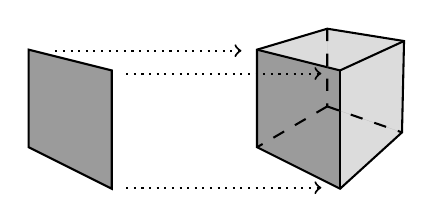
\begin{tikzpicture}[x=0.75pt,y=0.75pt,yscale=-1,xscale=1]
%uncomment if require: \path (0,300); %set diagram left start at 0, and has height of 300

%Shape: Polygon [id:ds6456828274457911] 
\draw  [draw opacity=0][fill={rgb, 255:red, 220; green, 220; blue, 220 }  ,fill opacity=1 ] (210.83,19.34) -- (209.85,63.35) -- (180,90.5) -- (140,70.5) -- (140,23.5) -- (173.85,13.4) -- cycle ;
%Shape: Polygon [id:ds680020141264005] 
\draw  [draw opacity=0][fill={rgb, 255:red, 155; green, 155; blue, 155 }  ,fill opacity=1 ] (140,23.5) -- (180,33.5) -- (180,90.5) -- (140,70.5) -- cycle ;
%Shape: Polygon [id:ds5687589405423901] 
\draw   (210.83,19.34) -- (209.85,63.35) -- (180,90.5) -- (140,70.5) -- (140,23.5) -- (173.85,13.4) -- cycle ;
%Straight Lines [id:da9469687653709942] 
\draw [fill={rgb, 255:red, 155; green, 155; blue, 155 }  ,fill opacity=1 ]   (140,23.5) -- (180,33.5) ;
%Straight Lines [id:da2062432509241826] 
\draw [fill={rgb, 255:red, 155; green, 155; blue, 155 }  ,fill opacity=1 ]   (180,33.5) -- (180,90.5) ;
%Straight Lines [id:da46744316613244596] 
\draw [fill={rgb, 255:red, 155; green, 155; blue, 155 }  ,fill opacity=1 ]   (180,33.5) -- (210.83,19.34) ;
%Straight Lines [id:da5416094663433387] 
\draw [fill={rgb, 255:red, 155; green, 155; blue, 155 }  ,fill opacity=1 ] [dash pattern={on 4.5pt off 4.5pt}]  (173.83,50.84) -- (140,70.5) ;
%Straight Lines [id:da5012793935921553] 
\draw [fill={rgb, 255:red, 155; green, 155; blue, 155 }  ,fill opacity=1 ] [dash pattern={on 4.5pt off 4.5pt}]  (173.83,50.84) -- (209.85,63.35) ;
%Straight Lines [id:da45641517444896496] 
\draw [fill={rgb, 255:red, 155; green, 155; blue, 155 }  ,fill opacity=1 ] [dash pattern={on 4.5pt off 4.5pt}]  (173.85,13.4) -- (173.83,50.84) ;
%Straight Lines [id:da7198388934354361] 
\draw  [dotted, ->] (77,35) -- (171,35) ;
%Shape: Polygon [id:ds3152112125064218] 
\draw  [fill={rgb, 255:red, 155; green, 155; blue, 155 }  ,fill opacity=1 ] (30,23.5) -- (70,33.5) -- (70,90.5) -- (30,70.5) -- cycle ;
%Straight Lines [id:da5715091044968261] 
\draw  [dotted, ->]  (77,90) -- (171,90) ;
%Straight Lines [id:da7956654320856] 
\draw  [dotted, ->]  (42.83,24) -- (132.5,24) ;

\end{tikzpicture}
\caption{Face map}
\label{fig:face-map}
\end{marginfigure}
% 
De Morgan algebras have two constants \( \izero \) and \( \ione \), 
representing the endpoints of the interval. They give rise to \emph{face maps},
that insert a constant in \( k \)-th position for all \( k \le n \):
% 
\begin{align*}
\mathrm{face}_{k,0}^n & := \langle x_1 , ...\ , x_{k-1} , \izero , x_{k} ...\ , x_n \rangle : \hom[\catCube]{n}{n+1} \\
\mathrm{face}_{k,1}^n & := \langle x_1 , ...\ , x_{k-1} , \ione , x_{k} ...\ , x_n \rangle : \hom[\catCube]{n}{n+1}
\end{align*}
% 
In the cubical set, \( X(\mathrm{face}_{k,0}^n) \) and 
\( X(\mathrm{face}_{k,1}^n) \) send a \( (n+1) \)-dimensional cube to its
``hyperfaces'', which are cubes of dimension n.
% 
Of course, by composing face maps in several 
dimensions, one can obtain faces of all dimensions \( k < n+1 \).

The cartesian structure of the cube category additionally gives rise to 
another similar family of maps from \( n \) to \( n+1 \), namely the
diagonal maps obtained by duplicating the \( k \)-th dimension:
\[
\mathrm{diag}_k^n := \langle x_1 , ...\ , x_k , x_k , ...\ , x_n \rangle : \hom[\catCube]{n}{n+1}
\]
\begin{marginfigure}[*-3]

\tikzset{every picture/.style={line width=0.75pt}} %set default line width to 0.75pt        

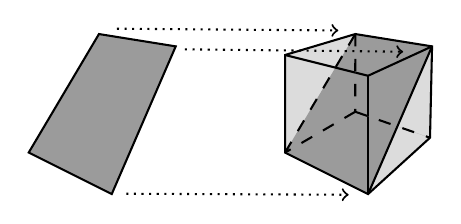
\begin{tikzpicture}[x=0.75pt,y=0.75pt,yscale=-1,xscale=1]
%uncomment if require: \path (0,300); %set diagram left start at 0, and has height of 300

%Shape: Polygon [id:ds5745484408615426] 
\draw  [draw opacity=0][fill={rgb, 255:red, 220; green, 220; blue, 220 }  ,fill opacity=1 ] (206.83,23.34) -- (205.85,67.35) -- (176,94.5) -- (136,74.5) -- (136,27.5) -- (169.85,17.4) -- cycle ;
%Shape: Polygon [id:ds06712756970437161] 
\draw  [draw opacity=0][fill={rgb, 255:red, 155; green, 155; blue, 155 }  ,fill opacity=1 ] (169.85,17.4) -- (206.83,23.34) -- (176,94.5) -- (136,74.5) -- cycle ;
%Shape: Polygon [id:ds5996187715144764] 
\draw   (206.83,23.34) -- (205.85,67.35) -- (176,94.5) -- (136,74.5) -- (136,27.5) -- (169.85,17.4) -- cycle ;
%Straight Lines [id:da4237123527435346] 
\draw [fill={rgb, 255:red, 155; green, 155; blue, 155 }  ,fill opacity=1 ]   (136,27.5) -- (176,37.5) ;
%Straight Lines [id:da781131552194921] 
\draw [fill={rgb, 255:red, 155; green, 155; blue, 155 }  ,fill opacity=1 ]   (176,37.5) -- (176,94.5) ;
%Straight Lines [id:da5908568759945031] 
\draw [fill={rgb, 255:red, 155; green, 155; blue, 155 }  ,fill opacity=1 ]   (176,37.5) -- (206.83,23.34) ;
%Straight Lines [id:da4718226705493266] 
\draw [fill={rgb, 255:red, 155; green, 155; blue, 155 }  ,fill opacity=1 ] [dash pattern={on 4.5pt off 4.5pt}]  (169.83,54.84) -- (136,74.5) ;
%Straight Lines [id:da6039581018465097] 
\draw [fill={rgb, 255:red, 155; green, 155; blue, 155 }  ,fill opacity=1 ] [dash pattern={on 4.5pt off 4.5pt}]  (169.83,54.84) -- (205.85,67.35) ;
%Straight Lines [id:da7974873720454588] 
\draw [fill={rgb, 255:red, 155; green, 155; blue, 155 }  ,fill opacity=1 ] [dash pattern={on 4.5pt off 4.5pt}]  (169.85,17.4) -- (169.83,54.84) ;
%Straight Lines [id:da8626821342091979] 
\draw    (176,94.5) -- (206.83,23.34) ;
%Straight Lines [id:da7109325118983972] 
\draw  [dash pattern={on 4.5pt off 4.5pt}]  (136,74.5) -- (169.85,17.4) ;
%Shape: Polygon [id:ds2989908540873938] 
\draw  [color={rgb, 255:red, 0; green, 0; blue, 0 }  ,draw opacity=1 ][fill={rgb, 255:red, 155; green, 155; blue, 155 }  ,fill opacity=1 ] (46.35,17.4) -- (83.33,23.34) -- (52.5,94.5) -- (12.5,74.5) -- cycle ;
%Straight Lines [id:da10251939706047508] 
\draw  [dotted, ->]  (55,14.83) -- (161.67,15.67) ;
%Straight Lines [id:da13820639137732804] 
\draw  [dotted, ->]  (87.75,24.75) -- (192.92,25.92) ;
%Straight Lines [id:da12067366869434382] 
\draw  [dotted, ->]  (59.5,94.33) -- (166.67,94.83) ;

\end{tikzpicture}
\caption{Diagonal map}
\label{fig:diagonal-map}
\end{marginfigure}
% 
One should think of these maps as embedding a \( n \)-dimensional cube
into the \( k \)-th main diagonal of a \( (n+1) \)-dimensional cube. 
We can get all the other diagonals by composing these maps with exchanges
and reversals.
% 
In a cubical set, the diagonal maps send cubes of dimension \( n+1 \) to
lower dimensional cubes, which should be pictured as their diagonals.
% 
\paragraph{Degeneracies and connections}
% 
If the cartesian structure of the cubes gave rise to \emph{duplication} maps,
it also gives rise to \emph{erasure} maps that delete the \( k \)-th 
coordinate: 
\[
\mathrm{degen}_k^n := \langle x_1 , ...\ , x_{k-1} , x_{k+1} , ...\ , x_n \rangle : \hom[\catCube]{n}{n-1}
\]
Such maps are called degenaracies, and should be pictured as squashing the
\( n \)-dimensional cube along the \( k \)-th dimension. Having these maps in
our cube category means that in a cubical set, a cube of dimension \( n \) 
comes with squashed cubes of all dimensions attached to it.
% 
This might appear strange at first glance, but one quickly realizes that it is
necessary: without degenerate cubes, it would be impossible to map the interval
to a point, since morphisms of cubical sets are natural transformations, which
must send 1-dimensional cubes to 1-dimensional cubes.
% 
With the degenerate cubes, it becomes possible: the 1-dimensional edge of the
interval is mapped to the degenerate edge contained in the 0-dimensional point.

\begin{figure}[!h]
\tikzset{every picture/.style={line width=0.75pt}} %set default line width to 0.75pt        

\begin{tikzpicture}[x=0.75pt,y=0.75pt,yscale=-1,xscale=1]
%uncomment if require: \path (0,300); %set diagram left start at 0, and has height of 300

%Shape: Rectangle [id:dp9618926780170471] 
\draw  [fill={rgb, 255:red, 155; green, 155; blue, 155 }  ,fill opacity=1 ] (20,20) -- (70,20) -- (70,70) -- (20,70) -- cycle ;
%Shape: Rectangle [id:dp43305185380684974] 
\draw  [color={rgb, 255:red, 180; green, 180; blue, 180 }  ,draw opacity=1 ][fill={rgb, 255:red, 230; green, 230; blue, 230 }  ,fill opacity=1 ] (100,30) -- (150,30) -- (150,60) -- (100,60) -- cycle ;
%Shape: Rectangle [id:dp2333548202396596] 
\draw  [color={rgb, 255:red, 180; green, 180; blue, 180 }  ,draw opacity=1 ][fill={rgb, 255:red, 230; green, 230; blue, 230 }  ,fill opacity=1 ] (180,40) -- (230,40) -- (230,50) -- (180,50) -- cycle ;
%Straight Lines [id:da8603874129078966] 
\draw    (260,45) -- (310,45) ;

%Straight Lines [id:da7040493759431076] 
\draw  [-latex']  (30,28) -- (30,62) ;
%Straight Lines [id:da9956574782521105] 
\draw  [-latex']  (60,28) -- (60,62) ;
%Straight Lines [id:da6148683812308081] 
\draw  [-latex'] (45,28) -- (45,62) ;

%Straight Lines [id:da4932670850314801] 
\draw [-latex', color={rgb, 255:red, 180; green, 180; blue, 180 }  ,draw opacity=1 ]   (110,35) -- (110,55) ;
%Straight Lines [id:da5868699666184711] 
\draw [-latex', color={rgb, 255:red, 180; green, 180; blue, 180 }  ,draw opacity=1 ]   (140,35) -- (140,55) ;
%Straight Lines [id:da3497854431759625] 
\draw [-latex', color={rgb, 255:red, 180; green, 180; blue, 180 }  ,draw opacity=1 ]   (125,35) -- (125,55) ;

%Straight Lines [id:da6973557709484423] 
\draw  [dotted, ->]  (80,45) -- (250,45) ;

\end{tikzpicture}
\caption{Graphical representation of the degeneracies}
\label{fig:degen}
\end{figure}
% 
Finally, the last family of maps come from the de Morgan binary operations
\( \lor \) and \( \land \), which correspond to the min and max operations 
on the real interval:
% 
\begin{align*}
\mathrm{join}_k^n & := \langle x_1 , ...\ , x_k \lor x_{k+1} , ...\ , x_n \rangle : \hom[\catCube]{n}{n-1} \\
\mathrm{meet}_k^n & := \langle x_1 , ...\ , x_k \land x_{k+1} , ...\ , x_n \rangle : \hom[\catCube]{n}{n-1}
\end{align*}
These maps are called \emph{connections}, and we can picture them as contracting 
a square onto its main diagonal, as if it were a folding fan (\cref{fig:connections}). In cubical sets,
connections equip cubes with two new families of degenerate cubes, allowing for
more maps between cubes. For now, connections may not seem as motivated as the
other operations, but they will play an important part in the next section, 
where we equip cubical sets with \emph{fibration structures}.

\begin{figure}[!h]
\tikzset{every picture/.style={line width=0.75pt}} %set default line width to 0.75pt        

\begin{tikzpicture}[x=0.75pt,y=0.75pt,yscale=-1,xscale=1]
%uncomment if require: \path (0,300); %set diagram left start at 0, and has height of 300

%Shape: Rectangle [id:dp1608426960338286] 
\draw  [fill={rgb, 255:red, 155; green, 155; blue, 155 }  ,fill opacity=1 ] (30,30) -- (80,30) -- (80,80) -- (30,80) -- cycle ;
%Straight Lines [id:da8693570671907255] 
\draw  [-latex']  (40,40) -- (65,40) ;
%Straight Lines [id:da9991679205274384] 
\draw  [-latex']  (40,50) -- (55,50) ;
%Straight Lines [id:da5399686539589947] 
\draw  [-latex']  (60,70) -- (60,55) ;
%Straight Lines [id:da7477537056366097] 
\draw  [-latex']  (70,70) -- (70,45) ;
%Straight Lines [id:da4174747849792645] 
% \draw    (30,90) -- (80,90) ;
%Straight Lines [id:da8922065987331226] 
% \draw    (20,80) -- (20,30) ;

%Shape: Polygon [id:ds6449189587092711] 
\draw  [draw={rgb, 255:red, 180; green, 180; blue, 180 } ,fill={rgb, 255:red, 230; green, 230; blue, 230 }  ,fill opacity=1 ] (130,30) -- (160,30) -- (160,60) -- (110,80) -- cycle ;
%Straight Lines [id:da9355184619004017] 
\draw  [-latex', draw={rgb, 255:red, 180; green, 180; blue, 180 }]  (132,40) -- (147,40) ;
%Straight Lines [id:da37227681217200015] 
\draw  [-latex', draw={rgb, 255:red, 180; green, 180; blue, 180 }]  (128,50) -- (138,50) ;
%Straight Lines [id:da6222003296136621] 
\draw  [-latex', draw={rgb, 255:red, 180; green, 180; blue, 180 }]  (150,58) -- (150,43) ;
%Straight Lines [id:da06324976564074081] 
\draw  [-latex', draw={rgb, 255:red, 180; green, 180; blue, 180 }]  (140,62) -- (140,52) ;

%Shape: Polygon [id:ds08647697638331286] 
\draw  [draw={rgb, 255:red, 180; green, 180; blue, 180 } ,fill={rgb, 255:red, 230; green, 230; blue, 230 }  ,fill opacity=1 ] (240,30) -- (240,40) -- (190,80) -- (230,30) -- cycle ;

%Straight Lines [id:da45075802478254534] 
\draw    (270,80) -- (320,30) ;

\draw  [dotted, ->]  (95,55) -- (265,55) ;

\node (lor) at (360,55) {``$x \lor y$''} ;

%Shape: Rectangle [id:dp6323071034180429] 
\draw  [fill={rgb, 255:red, 155; green, 155; blue, 155 }  ,fill opacity=1 ] (30,120) -- (80,120) -- (80,170) -- (30,170) -- cycle ;
%Straight Lines [id:da08953173271477399] 
\draw  [-latex']  (40,130) -- (40,155) ;
%Straight Lines [id:da241652915780334] 
\draw  [-latex']  (50,130) -- (50,145) ;
%Straight Lines [id:da5233837011369769] 
\draw  [-latex']  (70,160) -- (45,160) ;
%Straight Lines [id:da7482761157877976] 
\draw  [-latex']  (70,150) -- (55,150) ;
%Straight Lines [id:da43571360479866794] 
% \draw    (30,180) -- (80,180) ;
%Straight Lines [id:da7396310606195999] 
% \draw    (20,170) -- (20,120) ;

%Shape: Polygon [id:ds14683437162938429] 
\draw  [draw={rgb, 255:red, 180; green, 180; blue, 180 } ,fill={rgb, 255:red, 230; green, 230; blue, 230 }  ,fill opacity=1 ] (110,140) -- (160,120) -- (140,170) -- (110,170) -- cycle ;
%Straight Lines [id:da045896921256860845] 
\draw  [-latex', draw={rgb, 255:red, 180; green, 180; blue, 180 }]  (120,142) -- (120,157) ;
%Straight Lines [id:da3276251506585385] 
\draw  [-latex', draw={rgb, 255:red, 180; green, 180; blue, 180 }]  (130,138) -- (130,148) ;
%Straight Lines [id:da5143324187564968] 
\draw  [-latex', draw={rgb, 255:red, 180; green, 180; blue, 180 }]  (138,160) -- (123,160) ;
%Straight Lines [id:da20642737155806068] 
\draw  [-latex', draw={rgb, 255:red, 180; green, 180; blue, 180 }]  (142,150) -- (132,150) ;

%Shape: Polygon [id:ds32380308725317386] 
\draw  [draw={rgb, 255:red, 180; green, 180; blue, 180 } ,fill={rgb, 255:red, 230; green, 230; blue, 230 }  ,fill opacity=1 ] (240,120) -- (200,170) -- (190,170) -- (190,160) -- cycle ;

%Straight Lines [id:da19647470565636227] 
\draw    (270,170) -- (320,120) ;

\draw  [dotted, ->]  (95,145) -- (265,145) ;

\node (land) at (360,145) {``$x \land y$''} ;

\end{tikzpicture}
\caption{Graphical representation of the connections}
\label{fig:connections}
\end{figure}

As we can see, the functoriality condition translates this generating family of
\( \catCube \) into a family of operations on cubical sets. 
% 
Naturally, the equalities between morphisms in \( \catCube \) will translate
to \emph{equations} on these operations: reversals are idempotent, faces of 
degenerate cubes are themselves degenerate cubes, etc.
% 
All in all, this presheaf construction amounts to giving a multi-sorted, 
algebraic presentation of cubical sets.

% \subsection{Some examples of cubical sets}

% \paragraph{The Interval} 

% \begin{definition}
%     The interval \( \interval \) is the Yoneda embedding \( \yo(1) \)
%     of the interval from the cube category. 
% \end{definition}
% \sideremark{Recall that \( \yo(1)(n) = \hom[\catCube]{n}{1} \).} 
% The points of \( \interval \) are by definition the elements of 
% \( \hom[\catCube]{0}{1} \), that is \( \langle \izero \rangle \) and 
% \( \langle \ione \rangle \). 
 
% \begin{definition}
%     Let \( X \) be a cubical set, and \( x_1, x_2 \in X(0) \) be two points 
%     of \( X \). A path from \( x_1 \) to \( x_2 \) is a map from 
%     \( \interval \) to \( X \) that 
% \end{definition}

% The higher dimensional cubes of \( \interval \), however, are more 
% difficult to describe, because of the degeneracies and the connections.

% \shepherd{We can establish a graphical calculus to ``see'' the de Morgan
%     cubical sets. But is it really necessary...}

% \paragraph{The circle}

% \shepherd{TODO}

% \paragraph{Singular cubical sets}

% \shepherd{TODO}

\subsection{Fibrant Cubical Sets}

With cubical sets, we have a solid candidate for a combinatorial framework to
study spaces and deformations: cubical sets come equipped with notions of points, 
of paths, of 2-dimensional homotopies, etc.
% 
However, we are mising a crucial ingredient: the possibility to 
\emph{compose} paths and higher homotopies. Indeed, in a topological
space \( X \), given two paths \( p_1, p_2 : [0, 1] \to X \) with matching
endpoints, we can concatenate them as follows:
\[
    \begin{array}{lcl}
    p_1 \cdot p_2 & : & [0 , 1] \to X \\
    p_1 \cdot p_2 (x) & := &
        \left\{ 
            \begin{array}{ll} 
                p_1 (2x) & x \le 1/2 \\ 
                p_2 (2x - 1) & x > 1/2 
            \end{array} 
        \right. .
    \end{array}
\]
And likewise with higher-dimensional homotopies. However, in a cubical set
\( X \), there is seemingly no way to compose two paths from \( X(1) \) that 
have matching boundaries. 
% 
This is no small issue: without composition, we cannot even define the
fundamental group, a corner stone of homotopy theory!

We will remediate to this issue by equipping our cubical sets with 
\emph{fibration structures}, which are simply rules to compose cubes of
different dimension together.
% 
But before defining fibration structures, we need to work a bit more to
define what is a set of composable cubes.

% One of the most basic constructions in homotopy theory is the 
% \emph{fundamental group} of a space. 
% % 
% Given a topological space \( X \) and a point \( x_0 \in X \), the elements of
% its fundamental group \( \pi_1(X, x_0) \) are \defnote{loops}{A loop based at 
% \( x_0 \) is a continuous map \( \ell : [0, 1] \to X \) such that 
% \( \ell(0) = \ell(1) = x_0 \).} based at \( x_0 \) quotiented by
% \defnote{homotopy}{Two loops \( \ell_1 \) and \( \ell_2 \) are homotopic when 
% there is a continuous map \( h : [0, 1]^2 \to X \) such that 
% \( h(x, 0) = \ell_1(x) \) and \( h(x, 1) = \ell_2(x) \), as well as
% \( h(0, x) = h(1, x) = x_0 \) for all \( x \).}.
% % 
% The group law is given by concatenation: given two loops \( \ell_1 \) and 
% \( \ell_2 \), their concatenation is
% \[
%     \ell_1 \cdot \ell_2 (x) = 
%         \left\{ 
%             \begin{array}{ll} 
%                 \ell_1 (2x) & x \le 1/2 \\ 
%                 \ell_2 (2x - 1) & x > 1/2 
%             \end{array} 
%         \right. .
% \]

\begin{definition}
    The face lattice of dimension \( n \) is defined by
    \[
        \faces(n) := \hom[\catCube]{n}{1}
    \]
    or in other words, an element of \( \faces(n) \) is a term of
    \( \demorgan{x_1 , ... , x_n} \).
\end{definition}
% 
\begin{marginfigure}
\tikzset{every picture/.style={line width=0.75pt}} %set default line width to 0.75pt        

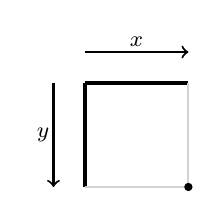
\begin{tikzpicture}[x=0.75pt,y=0.75pt,yscale=-1,xscale=1]
%uncomment if require: \path (0,300); %set diagram left start at 0, and has height of 300

\draw  [->]  (20,5) -- (70,5) ;
\node (x) at (45,0) {\footnotesize $x$} ;
\draw  [->]  (5,20) -- (5,70) ;
\node (y) at (0,45) {\footnotesize $y$} ;
%Straight Lines [id:da9288208803252698] 
\draw [line width=1.5]    (20,20) -- (70,20) ;
%Straight Lines [id:da9566129196020052] 
\draw [line width=1.5]    (20,20) -- (20,70) ;
%Straight Lines [id:da2609913656735583] 
\draw [color={rgb, 255:red, 210; green, 210; blue, 210 }  ,draw opacity=1 ]   (20,70) -- (70,70) ;
%Straight Lines [id:da8966542936579348] 
\draw [color={rgb, 255:red, 210; green, 210; blue, 210 }  ,draw opacity=1 ]   (70,20) -- (70,70) ;

\node [circle, fill=black, inner sep=0pt, minimum size=3pt] (A) at (70,70) {} ;
\end{tikzpicture}

\begin{small}
The element \( ({\sim} x) \lor ({\sim} y) \lor (x \land y) \) contains the
faces \( x = 0 \), \( y = 0 \) and \( (x = 1) \cap (y = 1) \).
\end{small}
\caption{An element of the face lattice}
    \label{fig:face-lattice}
\end{marginfigure}
% 
As the name suggests, morphisms of \( \hom[\catCube]{n}{1} \) can be used to
represent collections of faces of a cube of dimension \( n \). 
% 
The idea is simple: once put in disjunctive normal form, a term of 
\( \demorgan{x_1 , ... , x_n} \) can be described as a join of meets
of variables and negated variables.
% 
But if we replace \( x_i \) with \( x_i = 1 \) and \( {\sim} x_k \) with
\( x_k = 0 \), we can read that as a union of intersections of hyperfaces,
as in \cref{fig:face-lattice}.

Next, we associate an \emph{open box} to every element of the face lattice:

\begin{definition}
    Given \( f \in \faces(n) \), we build the open box \( \horn_f^n \) as
    a subobject of the \( (n+1) \)-dimensional cube \( \yo(n+1) \):
    \begin{align*}
        \horn_f^n(k) = & \{ x \in \hom[\catCube]{k}{n+1} \ |\ f \circ \mathrm{degen}_{n+1}^{n+1} \circ x = \ione \} \\
                     & \cup \{ x \in \hom[\catCube]{k}{n+1} \ |\ \pi_{n+1}\ x = \izero \}.
    \end{align*}
    In other words, we keep only the cubes whose first \( n \) coordinates
    belong to \( f \) and those whose last coordinate is \( \izero \).
\end{definition}
% 
\begin{marginfigure}


% Gradient Info
  
\tikzset {_w464gu8oa/.code = {\pgfsetadditionalshadetransform{ \pgftransformshift{\pgfpoint{0 bp } { 0 bp }  }  \pgftransformrotate{-310 }  \pgftransformscale{2 }  }}}
\pgfdeclarehorizontalshading{_fht55qnxt}{150bp}{rgb(0bp)=(0.69,0.69,0.69);
rgb(37.5bp)=(0.69,0.69,0.69);
rgb(62.5bp)=(0.44,0.44,0.44);
rgb(100bp)=(0.44,0.44,0.44)}

% Gradient Info
  
\tikzset {_93c71de5r/.code = {\pgfsetadditionalshadetransform{ \pgftransformshift{\pgfpoint{0 bp } { 0 bp }  }  \pgftransformrotate{-201 }  \pgftransformscale{2 }  }}}
\pgfdeclarehorizontalshading{_ubrxqtmte}{150bp}{rgb(0bp)=(0.69,0.69,0.69);
rgb(37.5bp)=(0.69,0.69,0.69);
rgb(62.5bp)=(0.44,0.44,0.44);
rgb(100bp)=(0.44,0.44,0.44)}
\tikzset{every picture/.style={line width=0.75pt}} %set default line width to 0.75pt        

\begin{tikzpicture}[x=0.75pt,y=0.75pt,yscale=-1,xscale=1]
%uncomment if require: \path (0,300); %set diagram left start at 0, and has height of 300

%Shape: Polygon [id:ds7637916967534137] 
\draw  [draw opacity=0][shading=_fht55qnxt,_w464gu8oa] (80.56,21.4) -- (80.54,71.79) -- (35,98.25) -- (35,34.99) -- cycle ;
%Shape: Polygon [id:ds8702408571107383] 
\draw  [draw opacity=0][shading=_ubrxqtmte,_93c71de5r] (80.56,21.4) -- (130.33,29.4) -- (129.01,88.63) -- (80.54,71.79) -- cycle ;
%Straight Lines [id:da5155765446101361] 
\draw [fill={rgb, 255:red, 155; green, 155; blue, 155 }  ,fill opacity=1 ]   (35,34.99) -- (35,98.25) ;
%Straight Lines [id:da5124304672404991] 
\draw [fill={rgb, 255:red, 155; green, 155; blue, 155 }  ,fill opacity=1 ]   (80.54,71.79) -- (35,98.25) ;
%Straight Lines [id:da45523551311619026] 
\draw  [dash pattern={on 4.5pt off 4.5pt}]  (80.54,71.79) -- (80.56,21.4) ;
%Straight Lines [id:da7921027264122242] 
\draw    (80.54,71.79) -- (129.01,88.63) ;
%Straight Lines [id:da5103415878863075] 
\draw    (130.33,29.4) -- (129.01,88.63) ;
%Straight Lines [id:da1999187844332465] 
\draw    (129.01,88.63) -- (88.84,125.17) ;
%Straight Lines [id:da8263212075628548] 
\draw    (80.54,71.79) -- (80.55,46.6) ;
%Shape: Polygon [id:ds08263649323643296] 
\draw  [draw opacity=0][fill={rgb, 255:red, 189; green, 189; blue, 189 }  ,fill opacity=1 ] (80.56,21.4) -- (130.33,29.4) -- (88.84,48.45) -- (35,34.99) -- cycle ;
%Straight Lines [id:da2367652420687777] 
\draw [fill={rgb, 255:red, 155; green, 155; blue, 155 }  ,fill opacity=1 ]   (35,34.99) -- (88.84,48.45) ;
%Straight Lines [id:da5190970570306638] 
\draw [fill={rgb, 255:red, 155; green, 155; blue, 155 }  ,fill opacity=1 ]   (88.84,48.45) -- (130.33,29.4) ;
%Straight Lines [id:da21329815944530717] 
\draw    (80.56,21.4) -- (130.33,29.4) ;
%Straight Lines [id:da22017891266687617] 
\draw    (35,34.99) -- (80.56,21.4) ;
%Straight Lines [id:da8474532817729444] 
\draw  [->]  (184.06,21.4) -- (211.33,27.17) ;
\node (x) at (211.33,21.17) {\footnotesize $x$} ;
%Straight Lines [id:da07666755630743649] 
\draw  [->]  (184.06,21.4) -- (167.33,32.17) ;
\node (z) at (167.33,25.17) {\footnotesize $z$} ;
%Straight Lines [id:da6791195518725582] 
\draw  [->] (184.06,21.4) -- (184.33,51.17) ;
\node (y) at (190.33,51.17) {\footnotesize $y$} ;
\end{tikzpicture}
\caption{The open box corresponding to \( ({\sim} x) \lor ({\sim} y) \lor (x \land y) \)
    is a subobject of the three-dimensional cube}
    \label{fig:open-box}
\end{marginfigure}
% 
% Alternatively, the open box \( \horn_f^n \) can be obtained by first taking the
% cartesian product \( f \times \interval \), and then adding a 
% \( n \)-dimensional lid.

Open boxes represent the shapes that can be composed together. Note
that the shape of two paths with matching endpoints is a special case of an 
open box: we can simply take \( \horn_{\langle x \rangle}^1 \).

Given an open box \( \horn_f^n \) and a cubical set \( X \), we define an
open box embedded in \( X \) to be a homomorphism of cubical sets \( \theta : \horn_f^n \to X \). 
Then, given a morphism \( \alpha : \hom[\catCube]{k}{n} \), we can extend the restriction
operation \( X(\alpha) \) to the open boxes embedded in \( X \) by applying 
\( \alpha \) to the first \( n \) coordinates of the open box.

\begin{definition}
    A CCHM fibration structure for a cubical set \( X \) is a function \( \Phi \) that takes
    as inputs an open box \( \theta : \horn_f^n \to X \) 
    and returns a ``lid'' \( \Phi(\theta) : \yo(n) \to X \) such that
    \begin{itemize}
        \item the lid matches the top of the open box, \ie
        \( \Phi(\theta)  \circ \mathrm{face^n_{n,1}}\) and \( \theta \) coincide 
        when they are both defined.
        \item  given any morphism \( \alpha : \hom[\catCube]{k}{n} \),
            the result of applying \( \Phi \) to the sub-open-box of \( \theta \) 
             \( f \circ \alpha \) is equal to the result of applying \( \Phi \)
            to the entire open box and restricting the result along \( \alpha \).
    \end{itemize}
\end{definition}

The map \( \theta : \horn_f^n \to X \) embeds an open box in \( X \), that is a
set of composable cubes, and the lid of the closed box \( \Phi(\theta) \)
represents the result of the composition.

\begin{figure}[!h]
    \tikzset{every picture/.style={line width=0.75pt}} %set default line width to 0.75pt        
    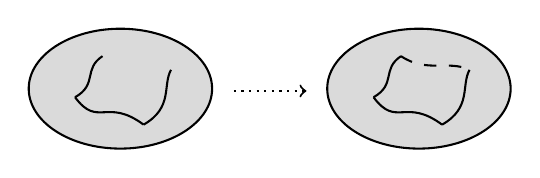
\begin{tikzpicture}[x=0.75pt,y=0.75pt,yscale=-1,xscale=1]
    %uncomment if require: \path (0,300); %set diagram left start at 0, and has height of 300
    
    %Shape: Ellipse [id:dp9399291638074402] 
    \draw  [fill={rgb, 255:red, 218; green, 218; blue, 218 }  ,fill opacity=1 ] (160,48.88) .. controls (160,32.93) and (179.78,20) .. (204.18,20) .. controls (228.58,20) and (248.37,32.93) .. (248.37,48.88) .. controls (248.37,64.83) and (228.58,77.76) .. (204.18,77.76) .. controls (179.78,77.76) and (160,64.83) .. (160,48.88) -- cycle ;
    %Curve Lines [id:da5142375426878248] 
    \draw    (182.33,53.02) .. controls (193.36,67.89) and (197.52,53.02) .. (215.35,66.22) ;
    %Curve Lines [id:da610717092369903] 
    \draw    (195.54,33.21) .. controls (186.1,39.5) and (193.36,46.76) .. (182.33,53.02) ;
    %Curve Lines [id:da8610634873385357] 
    \draw    (215.35,66.22) .. controls (229.68,57.99) and (224.4,47.42) .. (228.56,39.81) ;
    %Curve Lines [id:da31139389550283514] 
    \draw  [dash pattern={on 4.5pt off 4.5pt}]  (195.54,33.21) .. controls (207.89,41.53) and (218.45,34.92) .. (228.56,39.81) ;
    %Shape: Ellipse [id:dp6377592938264053] 
    \draw  [fill={rgb, 255:red, 218; green, 218; blue, 218 }  ,fill opacity=1 ] (16.18,48.88) .. controls (16.18,32.93) and (35.96,20) .. (60.36,20) .. controls (84.76,20) and (104.54,32.93) .. (104.54,48.88) .. controls (104.54,64.83) and (84.76,77.76) .. (60.36,77.76) .. controls (35.96,77.76) and (16.18,64.83) .. (16.18,48.88) -- cycle ;
    %Curve Lines [id:da5001632007053249] 
    \draw    (38.51,53.02) .. controls (49.54,67.89) and (53.7,53.02) .. (71.53,66.22) ;
    %Curve Lines [id:da16978501653986733] 
    \draw    (51.72,33.21) .. controls (42.27,39.5) and (49.54,46.76) .. (38.51,53.02) ;
    %Curve Lines [id:da6882456089332343] 
    \draw    (71.53,66.22) .. controls (85.85,57.99) and (80.57,47.42) .. (84.73,39.81) ;
    %Straight Lines [id:da7750254970630134] 
    \draw  [dotted, ->]  (115,50) -- (150,50) ;
    \end{tikzpicture}    
    % \caption{A fibrant cubical set: if we can draw an open box in \( X \), then we can close that box.}
    \label{fig:fibrant-space}
\end{figure}

\sideremark{There are many possible choices for what it means to ``compose'' 
    cubes, which translate to various fibration structures. In this thesis, we
    follow the CCHM paper \cite{CCHM}, so we will only care about CCHM-fibrant
    cubical sets.}
A cubical set equipped with a CCHM fibration structure is said to be 
\emph{CCHM-fibrant} (or just fibrant for short).

% \subsection{Examples of Fibrant Cubical Sets}

% \shepherd{TODO}

\subsection{Taking a Step Back}

With fibrant cubical sets, we have finally arrived at what seems to be a solid 
combinatorial framework for homotopy theory: 
% 
on the one hand, the category of de Morgan cubes and the fibration structures 
are elementary, constructive and amenable to computational methods;
% 
and on the other hand, fibrant cubical sets experimentally seem to behave just like 
``well-behaved'' topological spaces when considered up to deformation. As we
will see in \cref{ch:homotopy}, it is actually possible to define plenty of homotopical
constructions such as fundamental groups, homotopy pushouts, spheres, suspensions, 
or even the Hopf fibration.

While this is comforting, it would be more satisfying to have a mathematical 
result that connects the category of topological spaces and the category of
cubical sets ``up to deformation''. 
% 
\sideremark{It is however known that the geometric realization of CCHM-fibrant
    cubical sets is not a left Quillen adjunct \cite{QuillenDiscussion}. 
    But Quillen adjunctions are less general than higher equivalences.}
The adequate framework to formalize and prove such theorems is \emph{higher 
category theory}. Unfortunately, to the best of our knowledge, the problem of 
whether CCHM-fibrant cubical sets and well-behaved topological spaces are 
equivalent higher categories is still open as of today.

The reader who wishes to learn more about combinatorial methods in homotopy 
theory is invited to consult \sidecitet{friedmanSsets}, which treats the case 
of \emph{simplicial} sets (which are built out of simplices instead of cubes) in a 
similarly elementary manner, in greater detail.

\section{Toward a Cubical Translation}
\label{sec:cubical_trans}

We now turn ourselves to the task of translating 
\defnote{\( \MLTT{+}\mathsf{Univalence} \)}{The system \( \MLTT{+}\mathsf{Univalence} \) is defined to be 
Martin-Löf type theory extended with the univalence axiom, without the
computation rule for the \( J \) eliminator on reflexivity.} 
into a simpler type theory.
% 
Our strategy is to use the prefascist translation of Pédrot~\cite{pedrot:prefascist}  
to get an interpretation of \( \MLTT \) in the category of cubical sets, and 
then to extend it with CCHM fibration structures.

The translation of Pédrot uses 
\defnote{\( \sMLTT \)}{\( \sMLTT \) extends \MLTT with strict propositions, and 
an inductive equality valued in strict propositions \emph{à la} \Lean.} as its target 
type theory, as it relies on proof-irrelevant propositions and a proof-irrelevant
equality type with large elimination.
% 
For our part, we also want to have function extensionality in order to deal with 
fibration structures.
% 
This would make \SetoidCC a natural choice for our target type theory, 
but we also need the \( J \) eliminator to compute on reflexivity---which means
we actually need to use the extended system \SetoidCCplus (see \cref{sec:cast-refl}).

As we will realize shortly, the definition of a fibration structure 
will involve complex constructions in the language of \SetoidCCplus.
% 
To make sure that we are not overlooking some important type dependency or some 
missing computation rule, it seems reasonable to define our translation with the help of a 
proof assistant.
% 
We opt for \Agda, since we can use its proof-irrelevant propositions and rewrite 
rules~\sidecite{taming_of_the_rew} to support the theory of \SetoidCCplus.
% 
Thus all the \Agda code in this section uses the theory of \SetoidCCplus, which
means that we have access to the observational equality 
\AgdaBound{a}~\func{\textasciitilde{}}~\AgdaBound{b} and the \func{cast} operator.


\subsection{Defining the Category of Cubes in Type Theory}

The first step is to define the category of de Morgan cubes as a \emph{strict}
category, \ie as a category with a composition
operation that satisfies the associativity law and the unit laws up to a 
definitional equality.
% 
We could define this category in \SetoidCCplus by using the quotient
types to define de Morgan algebras, and then using the Yoneda embedding to
strictify the resulting category as explained in \cref{sec:cat-strictification}.

\begin{marginfigure}
\begin{tikzcd}
& i_1 \ar[dash]{dr} \ar[dash]{dl} & \\
i_l \ar[dash]{dr} & & i_r \ar[dash]{dl} \\
& i_0 &
\end{tikzcd}
\caption{The diamond algebra \( \mathbb{D} \)}
\end{marginfigure}
% 
However, we can devise a much simpler embedding of the category of de Morgan
cubes in the category of types and functions:
% 
define the \emph{diamond algebra} \( \mathbb{D} \) as the de Morgan algebra with carrier set 
\( \{ i_0, i_l, i_r, i_1 \} \) where the meet, join and reversal are defined by 
the four equations
\begin{mathpar}
i_l \vee i_r = i_1
\and i_l \wedge i_r = i_0 
\and \sim i_l = i_l 
\and \sim i_r = i_r. 
\end{mathpar}
% 
Then two morphisms \( f, g \in \hom[\catCube]{m}{n} \) in the category of de 
Morgan cubes are equal if and only if their interpretation as functions of type 
\( \mathbb{D}^m \to \mathbb{D}^n \) are pointwise equal~\sidecite{demorgan}.
% 
This implies that we can define the hom-sets of the category of cubes as 
subsets of function types, so that composition of morphisms coincides 
with function composition and the identity morphism coincides with the 
identity function.

Consequently, we define an inductive type of codes for morphisms, using the
generating family that we described in the previous section: 

\ExecuteMetaData[chapters/literate-agda/Translation.tex]{demorgan}

Then, we define the interpretation of a code as a function on the diamond
algebra:

\ExecuteMetaData[chapters/literate-agda/Translation.tex]{demorganinterp}

And finally, we define the type of morphisms \( \hom[\catCube]{n}{m} \) as the 
type of pairs of a diamond algebra function and a proof that it corresponds to
the interpretation of a code.

\ExecuteMetaData[chapters/literate-agda/Translation.tex]{category}

Note that the field \field{code} is proof-irrelevant.
% 
If our records satisfy the \( \eta \)-rule, this implies that morphisms behave
exactly like functions and thus that they are definitionally associative.

% something about supplementary equations?

\subsection{The Universe of Cubical Sets}

Now that we have our strict category of de Morgan cubes, we can set the stage 
for the prefascist translation. Recall the definition 
of prefascist types from \cref{ch:prefascist}:

\ExecuteMetaData[chapters/literate-agda/Translation.tex]{prefascist}

If we want to use these to build a model of univalent type theory, we first 
need to define a handful of building blocks.
% 
We start with a hierarchy of prefascist types indexed by a level \( \ell \) 
that plays the role of a universe hierarchy for the category of prefascist types.
 
From the work of Hofmann and Streicher on presheaf 
universes~\sidecite{HofmannStreicher}, we know that the type of sections of a 
universe over an object \( n \) should be the type of prefascist types on the 
% 
\defnote{slice category}{The slice category over an object \( n \) is noted
\( \catCube_{/n} \). The objects of the slice category are the morphisms of 
\( \catCube \) with codomain \( n \), and a morphism of the slice category 
from \( f : a \to n \) to \( g : b \to n \) is a \( h : a \to b \) such that 
\( g \circ h = f \).} 
% 
\( \catCube_{/n} \):

\ExecuteMetaData[chapters/literate-agda/Translation.tex]{yt}

This type family will fill the role of the field \field{F₀} for our universal 
prefascist.
% 
Note that it has a natural restriction operation: given \( \alpha : \func{Hom}~m~n \), 
we can define restriction as composition with \( \alpha \) in both fields.
% 
\sideremark{Recall that we defined the notation \( α~\func{∙}~x \) as a shorthand for
\( λ~\AgdaBound{m'}~\AgdaBound{α'}~\func{→}~x~\AgdaBound{m'}~(α~\func{∘}~\AgdaBound{α'}) \). }
% 
\begin{code}
\>[0]\func{restr}~\AgdaSymbol{:}~(\AgdaBound{α}~\AgdaSymbol{:}~\func{Hom}~\AgdaBound{m}~\AgdaBound{n})~%
\AgdaSymbol{→}~(\func{cubicalType₀}~\AgdaBound{ℓ}~\AgdaBound{n})~%
\AgdaSymbol{→}~(\func{cubicalType₀}~\AgdaBound{ℓ}~\AgdaBound{m})\<%
\\
\>[0]\func{restr}~\AgdaBound{α}~(\con{CT}~\AgdaBound{ct0}~\AgdaBound{ctε})~%
\AgdaSymbol{=}~\con{CT}~(\AgdaBound{α}~\func{∙}~\AgdaBound{ct0})~(\AgdaBound{α}~\func{∙}~\AgdaBound{ctε})\<%
\end{code}

Now we can use this restriction operator to devise a predicate \func{cubicalTypeε} 
on families of sections of \func{cubicalType₀}, that will be the field \field{Fε} of the 
universal prefascist type.

\ExecuteMetaData[chapters/literate-agda/Translation.tex]{cubicaleps}

And thus we can define the universal prefascist type \( \func{cubicalType}~\ell \).
% 
\begin{code}
\>[0]\func{cubicalType}~\AgdaSymbol{:}~\AgdaSymbol{∀}~\AgdaBound{ℓ}~\AgdaSymbol{→}~\func{prefascist}\<%
\\
\>[0]\func{cubicalType}~\AgdaBound{\ell}~%
\AgdaSymbol{=}~\AgdaSymbol{\{}~\field{F₀}~\AgdaSymbol{=}~\func{cubicalType₀}~\AgdaBound{ℓ}~\AgdaSymbol{;}~%
\field{Fε}~\AgdaSymbol{=}~\func{cubicalTypeε}~\AgdaSymbol{\}}\<%
\end{code}

This universe hierarchy allows us to model \emph{dependent types} in the 
category of prefascist types: given a prefascist \( A \), a dependent prefascist
on \( A \) is a prefascist morphism from \( A \) to \func{cubicalType}.
% 
Furthermore, if we have a prefascist morphism \( B \to A \) and a dependent prefascist type
on \( A \), we can get a dependent prefascist type on \( B \) with a simple 
morphism composition.
% 
This ``substitution'' operation is strictly associative, which is very important when it
comes to building models of dependent type theory~\sidecite{Hofmann97}.

% Now, let's unfold this definition a little bit: if \( A \) is a prefascist type, 
% then a dependent prefascist on \( A \) is the data of 

\subsection{Fibration Structures}

However, the model of Cohen \etal does not only interpret types as arbitrary
cubical presheaves, it also equips them with fibration structures.
% 
We want to equip our dependent prefascist types with analogous 
fibration structures, which means that we need to build a universe of 
\emph{CCHM-fibrant} prefascist types. 

Its type of sections is defined as follows:
% 
\sideremark[*5]{Given a morphism \( α : \hom[\catCube]{n}{1} \) in the category of 
    cubes, or equivalently an element of the lattice of faces of the cube of 
    dimension \( n \), the proposition \( \func{is⊤}~\alpha \) is true when
    \( \alpha \) is the maximal element of the face lattice. This proposition 
    supports a restriction operation, that we write \func{restr}.}
% 
\sideremark[*18]{The morphisms \func{side0}, \func{side1}, \func{degen} 
    correspond respectively to \( \mathrm{face}_{0,0}^n \), \( \mathrm{face}_{0,1}^n \)
    and \( \mathrm{degen}_{0}^n \) from the previous section.}
% 
\sideremark[*23]{Given a morphism \( α : \hom[\catCube]{m}{n} \) in the category
    of cubes, the morphism \( \func{lift}~α : \hom[\catCube]{m+1}{n+1} \) is the
    identity on the first coordinate and is equal to \( α \) on the remaining 
    coordinates.}
% 
\ExecuteMetaData[chapters/literate-agda/Translation.tex]{yft}

Just like in the type \func{cubicalType₀}, the fields \field{FT₀} and
\field{FTε} define a prefascist type on the category \( \catCube_{/n} \), or
equivalently a prefascist indexed over \( \yo~n \) by the Yoneda lemma.

The fields \field{comp₀}, \field{compε} and \field{comp\textasciitilde{}} compute 
a lid for an arbitrary open box in the dependent prefascist, which corresponds 
to the (non-homogeneous) composition in CCHM cubical type theory. 
Their arguments are
% 
\begin{itemize}
\item a morphism \( \alpha \) that embeds a cube of dimension \( m+1 \)
in \( \yo~n \) and an element of the face lattice \( \varphi \), which 
together define an open box \( \theta : \horn^m_\varphi \to \yo~n \) ;
\item an element of the dependent prefascist retricted to the sides the open 
box \( \theta \), given by \AgdaBound{p0} and \AgdaBound{pε} ;
\item an element of the dependent prefascist restricted to the bottom of the
open box \( \theta \), given by \AgdaBound{s0} and \AgdaBound{sε} ; and
\item a proof that the elements on the sides and on the bottom coincide,
given by \AgdaBound{s\textasciitilde}.
\end{itemize}
% 
From these, \field{comp₀} computes an element of \field{FT₀} over the lid of
the open box. The field \field{compε} ensures that restricting a lid is
the same as computing a lid for the restricted box, and \field{comp\textasciitilde{}}
ensures that the lid coincides with the sides of the box when both are defined.

Just like the type \func{cubicalType₀}, our type \func{fibrantType₀} admits a 
natural restriction operation derived from composition.
% 
From this restriction operation, we define the predicate \func{fibrantTypeε} as 
follows
% 
\ExecuteMetaData[chapters/literate-agda/Translation.tex]{fibranteps}
% 
And finally, we can define the prefascist \func{fibrantType}.
% 
\begin{code}
\>[0]\func{fibrantType}~\AgdaSymbol{:}~\func{prefascist}\<%
\\
\>[0]\func{fibrantType}~%
\AgdaSymbol{=}~\AgdaSymbol{\{}~\field{F₀}~\AgdaSymbol{=}~\func{fibrantType₀}~\AgdaSymbol{;}~%
\field{Fε}~\AgdaSymbol{=}~\func{fibrantTypeε}~\AgdaSymbol{\}}\<%
\end{code}

\subsection{Building a Model as a Translation}
\label{sec:trans-overview}

We can extract a model of dependent type theory from the universe \func{fibrantType}
by interpreting contexts as telescopes of dependent prefascist types, types as 
dependent prefascist types, and terms as sections.

We phrase this model as a syntactic translation, \ie as a family of functions
from the syntax of \MLTT to the syntax of \SetoidCCplus:
% 
\begin{itemize}
\item To every context of \MLTT terms \( \Gamma \), we associate a family of contexts of \SetoidCCplus
    indexed by an object \( n : \func{Obj} \), that we write \( \llbracket Γ \rrbracket^n \).
\item To every term \( t \) of \MLTT, we associate two families of terms
    % \( \llbracket t \rrbracket^n_0 \), \( \llbracket t \rrbracket^n_ε \), 
    \( {[t]}^n_0 \) and \( {[t]}^n_ε \) indexed by an object \( n : \func{Obj} \).
\end{itemize}

\begin{figure}
\begin{small}
\[
\begin{array}{lcl}
{[x]}^n_0 & := & x_0 \\
{[x]}^n_ε & := & x_ε 
\vspace{0.5em}\\
{[λ(x:A)~.~t]}^n_0 & := & λ~m~α~x_0~x_ε~.~{[t]}^m_0~x_0~x_ε~m~(\func{id}~m)\\ 
{[λ(x:A)~.~t]}^n_ε & := & λ~m~α~x_0~x_ε~.~{[t]}^m_ε~x_0~x_ε~m~(\func{id}~m)
\vspace{0.5em}\\
{[t~u]}^n_0 & := & λ~m~α~.~{[t]}^n_0~m~α~(α\cdot{[u]}^n_0)~(α\cdot{[u]}^n_ε)\\
{[t~u]}^n_ε & := & λ~m~α~.~{[t]}^n_ε~m~α~(α\cdot{[u]}^n_0)~(α\cdot{[u]}^n_ε)
\vspace{0.5em}\\
{[A \to B]}^n_0 & := & \func{Arr₀}~{[A]}^n_0~{[A]}^n_ε~{[B]}^n_0~{[B]}^n_ε\\
{[A \to B]}^n_ε & := & \func{Arrε}~{[A]}^n_0~{[A]}^n_ε~{[B]}^n_0~{[B]}^n_ε
\vspace{0.5em}\\
{[\Pi (x : A)~.~B]}^n_0 & := & \func{Prod₀}~{[A]}^n_0~{[A]}^n_ε~{[B]}^n_0~{[B]}^n_ε\\
{[\Pi (x : A)~.~B]}^n_ε & := & \func{Prodε}~{[A]}^n_0~{[A]}^n_ε~{[B]}^n_0~{[B]}^n_ε
\vspace{0.5em}\\
{[\mathsf{Type}]}^n_0 & := & \func{fType₀}\\
{[\mathsf{Type}]}^n_ε & := & \func{fTypeε}\\
% \\
% {\llbracket A\rrbracket}^n_0 & := & \func{El₀}~{[A]}^n_0 \\
% {\llbracket A\rrbracket}^n_ε & := & \func{Elε}~{[A]}^n_0~{[A]}^n_ε \\
\\
\llbracket \emptyctx \rrbracket^n & := & n : \func{Obj} \\
\llbracket \Gamma,~x:A \rrbracket^n & := & \llbracket \Gamma \rrbracket^n~,~x_0:\func{El₀}~{[A]}^n_0~,~x_ε:\func{Elε}~{[A]}^n_0~{[A]}^n_ε~x_0
\end{array}
\]
\end{small}
\caption{Core of the fibrant prefascist translation}
\label{fig:prefascist-trans}
\end{figure}

The intuition behind these functions is that if \( A \) is a type of \MLTT in 
context \( \Gamma \), then the two following judgments should be derivable in
\SetoidCCplus: 
\[
\begin{array}{lclcl}
\llbracket Γ \rrbracket^n & \vdash & {[ A ]}^n_0 & : & 
\AgdaSymbol{∀}~\AgdaBound{m}~%
\AgdaSymbol{(}\AgdaBound{α}~\AgdaSymbol{:}~\AgdaRecord{Hom}~\AgdaBound{m}~\AgdaBound{n}\AgdaSymbol{)}~%
\AgdaSymbol{→}~\AgdaRecord{fibrantType₀}~\AgdaBound{m}\\
\llbracket Γ \rrbracket^n & \vdash & {[ A ]}^n_ε & : &
\AgdaSymbol{∀}~\AgdaBound{m}~%
\AgdaSymbol{(}\AgdaBound{α}~\AgdaSymbol{:}~\AgdaRecord{Hom}~\AgdaBound{m}~\AgdaBound{n}\AgdaSymbol{)}~%
\AgdaSymbol{→}~\AgdaRecord{fibrantTypeε}~(\AgdaBound{α}~\func{∙}~{[ A ]}^n_0)
\end{array}
\]

Taken together, these judgments encode an element of \func{fibrantType}, or in other words a prefascist type
that depends on \( \llbracket Γ \rrbracket^n \).

If the judgment \( \Gamma \vdash t : A \) is derivable in \MLTT,
\( {[t]}^n_0 \) and \( {[t]}^n_ε \) should correspond to a section of
the prefascist type associated with \( A \).
% 
To define this type of sections, we introduce the following two functions:
%  
\sideremark[*7]{Here, we need to use a \func{cast} to convert between sections
of \AgdaBound{A0}~\AgdaBound{m'}~(\AgdaBound{α}~\func{∘}~\AgdaBound{α'}) and
sections of \AgdaBound{A0}~\AgdaBound{m}~\AgdaBound{α}.
Similar type-castings will come up frequently, so we will abreviate them as
\func{pfcast} from now on.}
% 
\ExecuteMetaData[chapters/literate-agda/Translation.tex]{elzero}

\ExecuteMetaData[chapters/literate-agda/Translation.tex]{elone}

And then, if the judgment \( \Gamma \vdash t : A \) is derivable in \MLTT,
we have
\[
\begin{array}{lclcl}
\llbracket Γ \rrbracket^n & \vdash & {[ t ]}^n_0 & : & \func{El₀}~{[ A ]}^n_0\\
\llbracket Γ \rrbracket^n & \vdash & {[ t ]}^n_ε & : & \func{Elε}~{[ A ]}^n_0~{[ A ]}^n_ε.
\end{array}
\]

The translation for a core type theory with function types, dependent products 
and one universe is given in \cref{fig:prefascist-trans}. 
% 
Ideally the universe should be translated as a fibrant prefascist type, but the 
definition of the fibration structure for the universe relies on 
\emph{Glue types} which are left for future work.
% 
For now, we interpret the universe a non-fibrant prefascist type instead:
% 
\sideremark{Since \func{fType₀} is not a fibrant prefascist type, the 
application \func{El₀}~\func{fType₀} is technically ill-typed.
To avoid wasting too much of our attention on this kind of annoyances, we will
silently extend \func{El₀} and \func{Elε} to non-fibrant prefascist
types.}

\begin{code}
\>[0] \func{fType₀}~:~\AgdaSymbol{∀}~\AgdaSymbol{\{} \AgdaBound{n} \AgdaSymbol{\}}~%
\AgdaBound{m}~\AgdaSymbol{→}~(\AgdaBound{α} : \func{Hom}~\AgdaBound{m}~\AgdaBound{n})~%
\AgdaSymbol{→}~\func{cubicalType₀}~\func{\_}~\AgdaBound{m} \<%
\\
\>[0] \func{fType₀}~\AgdaSymbol{\{} \AgdaBound{n} \AgdaSymbol{\}}~%
\AgdaBound{m}~\AgdaBound{α}~\AgdaSymbol{=}~\con{CT}~%
(\AgdaSymbol{λ}~\AgdaBound{m'}~\AgdaBound{α'}~\AgdaSymbol{→}~\func{fibrantType₀}~\AgdaBound{m'})\<%
\\
\>[0]\phantom{\func{fType₀}~\AgdaSymbol{\{} \AgdaBound{n} \AgdaSymbol{\}}~%
\AgdaBound{m}~\AgdaBound{α}~\AgdaSymbol{=}~\con{CT}}
(\AgdaSymbol{λ}~\AgdaBound{m'}~\AgdaBound{α'}~\AgdaBound{x}~\AgdaSymbol{→}~\func{fibrantTypeε}~\AgdaBound{x}) \<%
\end{code}

\begin{code}
\>[0] \func{fTypeε}~:~\AgdaSymbol{∀}~\AgdaSymbol{\{} \AgdaBound{n} \AgdaSymbol{\}}~%
\AgdaBound{m}~\AgdaSymbol{→}~(\AgdaBound{α} : \func{Hom}~\AgdaBound{m}~\AgdaBound{n})~%
\AgdaSymbol{→}~\func{cubicalTypeε}~(\AgdaBound{α}~\func{∙}~\func{fType₀}) \<%
\\
\>[0] \func{fTypeε}~\AgdaSymbol{\{} \AgdaBound{n} \AgdaSymbol{\}}~%
\AgdaBound{m}~\AgdaBound{α}~\AgdaBound{m'}~\AgdaBound{α'}~\AgdaSymbol{=}~\func{refl}
\end{code}

Without a fibration structure for the universe, we cannot eliminate the 
propositional equality in large types.

\subsection{Function Types and Dependent Products}

In order to interpret the function types, we replicate Pédrot's construction
and supplement it with a fibration structure adapted from the fibration 
structure of Cohen \etal
% 
\sideremark[*14]{\func{rev} is the morphism in the cube category that flips
the first coordinate. \func{empty} is the minimal element of the face lattice.
\func{∅} provides us with a partial element defined on \func{empty}.}

\ExecuteMetaData[chapters/literate-agda/Translation.tex]{arrzero}
% 
\sideremark[*-5]{For the sake of brevity, we omit the fields \field{compε} and 
    \field{comp\textasciitilde{}}, which are computationally irrelevant
    anyway.}

\ExecuteMetaData[chapters/literate-agda/Translation.tex]{arreps}

To define the \( λ \)-abstraction and the function application we can use the
exact same definitions as in the translation of Pédrot, since the fibration structure
is not involved.
% 
These definitions respect the \( \beta \) and \( \eta \) rules: assuming the
involved terms are well-typed, the interpretation of \( (λx\ .\ t)\ u \) is 
convertible to the interpretation of \( t[u/x] \), and the interpretation
of \( λx\ .\ t\ x \) is convertible to the interpretation of \( t \).

The construction for dependent products is very similar, if slightly more
complex. We have not verified it in a proof assistant yet.

\subsection{The Natural Numbers}

We can extend our core translation to support natural numbers.
We interpret the type of natural numbers as a constant prefascist, whose type of
sections is equal to \( \Nat \) in all dimensions. A family of sections is 
deemed compatible if they are all equal to the same natural number.

\ExecuteMetaData[chapters/literate-agda/Translation.tex]{natzero}

\ExecuteMetaData[chapters/literate-agda/Translation.tex]{nateps}

The composition operation is quite straightforward: an open box of natural 
numbers is necessarily constant, and thus the bottom element can serve as
a lid.

As shown by Pédrot, we can interpret 0, the successor function, and the
induction principle. Furthermore, the computation rule of the induction
principle is interpreted by a definitional equality.

\subsection{The Cubical Equality}

The interpretation of the propositional equality type is more 
interesting. We cannot add a fibration structure to the equality type used by Pédrot, 
since this type is not fibrant in general. 
% 
Instead we want to interpret an equality between \( x \) and \( y \) as a
\emph{path} from \( x \) to \( y \). 

In the cubical world, if \( x \) and
\( y \) are two \( n \)-dimensional sections of a prefascist type \( A \),
then a path should be a \( (n+1) \)-dimensional cube which has \( x \)
and \( y \) as opposing faces:

\ExecuteMetaData[chapters/literate-agda/Translation.tex]{cubeqzero}

This definition admits a natural restriction along morphisms of the cube 
category, that we (once again) write \func{restr}:

\begin{code}
\>[0]\func{restr}\ \AgdaSymbol{:}\ (\AgdaBound{α}\ \AgdaSymbol{:}\ \func{Hom}~\AgdaBound{m}~\AgdaBound{n})%
\ \AgdaSymbol{→}\ \func{cubicalPath}\ \AgdaBound{A0}\ \AgdaBound{Aε}\ \AgdaBound{x0}\ \AgdaBound{y0}\<%
\\
\>[0]\phantom{\func{restr}\ \AgdaSymbol{:}}
\AgdaSymbol{→}\ \func{cubicalPath}\ (\AgdaBound{α}~\func{∙}~\AgdaBound{A0})%
\ (\AgdaBound{α}~\func{∙}~\AgdaBound{Aε})%
\ (\AgdaBound{α}~\func{∙}~\AgdaBound{x0})%
\ (\AgdaBound{α}~\func{∙}~\AgdaBound{y0})\<%
\\
\>[0]\func{restr}~\AgdaBound{α}~(\con{CE}~\AgdaBound{ce0}~\AgdaBound{ceε}~\AgdaBound{lb}~\AgdaBound{rb})~\AgdaSymbol{=}~%
\con{CE}~(\func{lift}~\AgdaBound{α}~\func{∙}~\AgdaBound{ce0})~(\func{lift}~\AgdaBound{α}~\func{∙}~\AgdaBound{ceε})\<%
\\
\>[0]\hspace{11em}
(\func{ap}~(\AgdaSymbol{λ}~\AgdaBound{x}~\AgdaSymbol{→}~\AgdaBound{α}~\func{∙}~\AgdaBound{x})~\AgdaBound{lb})~%
(\func{ap}~(\AgdaSymbol{λ}~\AgdaBound{x}~\AgdaSymbol{→}~\AgdaBound{α}~\func{∙}~\AgdaBound{x})~\AgdaBound{rb})\<%
\end{code}

We use these to define the interpretation of the propositional equality.
\sideremark[*8]{The map \func{degen'}~:~\func{Hom}~(n+2)~(n+1) applies a 
degeneracy on the second coordinate, contrary to the map \func{degen} which
acts on the first coordinate.\\ 
The map \func{proj0}~:~\func{Hom}~(n+1)~1 is the projection of the first
coordinate.
The operator \func{merge} takes a partial element on face \AgdaBound{φ} 
and a partial element on face \AgdaBound{ψ} which are compatible on
\AgdaBound{φ}~\func{∧}~\AgdaBound{ψ} and produces a partial element on
face \AgdaBound{φ}~\func{∨}~\AgdaBound{ψ} (in our case, it is generalized to three arguments).}

\ExecuteMetaData[chapters/literate-agda/Translation.tex]{eqzero}

We could have hoped to derive the fibration structure of the equality type 
from that of \AgdaBound{A0} with a few algebraic manipulations, but it turns
out to be surprisingly nontrivial because of the boundary conditions.

The proof of reflexivity is derived from a degeneracy morphism: 

\ExecuteMetaData[chapters/literate-agda/Translation.tex]{reflzero}

and \func{eqreflε} is given by reflexivity.

In order to interpret the \( J \) eliminator, we break it into 
transport and contractibility of the singletons, following Cohen \etal
% 
The former can be derived from the fibration structure of the types, and the
latter can be proved with the structure of the category of cubes and some
heavy boundary condition yoga.
% 
We omit the proofs, as they get quite verbose.

Additionally, we were able to formally verify a proof of function 
extensionality, which can be derived without proving the univalence axiom.

\subsection{Glue Types}

So far, we have the elementary bricks of \MLTT down: a universe of fibrant types,
dependent products, natural numbers, and a propositional equality.
% 
However, our initial goal was to interpret the univalence axiom. How should we go 
about that?

In the model of Cohen \etal, this relies on \emph{Glue types}, a construction 
that can be used to replace faces of a cubical presheaf with equivalent types.
% 
It seems clear that Glue types can be adapted to the world of fibrant prefascist 
types given the similarity with presheaves, but we have not formalized it yet.

Furthermore, Glue types allow us to define the fibration structure for the 
universe. As such, they are the obvious next step in this line of research.

\section{Consequences and Perspectives}
\label{sec:cubical-perspectives}

Our prefascist translation is not quite complete as it stands, but it hopefully 
makes a strong argument for the possibility to translate 
\( \MLTT{+}\mathsf{Univalence} \) into \SetoidCCplus.
% 
In this section, we investigate the theoretical consequences of such a 
translation, if it were completed.

\subsection{The system \HoTTminus}

Assume that we have an extension of the functions \( {[\_]}^n_0 \) and
\( {[\_]}^n_ε \) from \cref{sec:trans-overview} to the full syntax of 
\( \MLTT{+}\mathsf{Univalence} \), such that
\begin{itemize}
\item Given any typing judgment \( \Gamma \vdash t : A \) that is derivable in 
\( \MLTT{+}\) \(\mathsf{Univalence} \), the translated judgments are derivable in 
\SetoidCCplus:
\[
\begin{split}
\llbracket \Gamma \rrbracket^n & \vdash {[t]}^n_0 : \func{El₀}~{[A]}^n_0 : \Type \\
\llbracket \Gamma \rrbracket^n & \vdash {[t]}^n_ε : \func{Elε}~{[A]}^n_0~{[A]}^n_ε~{[t]}^n_0 : \sProp
\end{split}
\]
\item Given any convertibility judgment \( \Gamma \vdash t \equiv u : A \) that is 
derivable in \( \MLTT{+}\) \(\mathsf{Univalence} \), the translated judgment is 
derivable in \SetoidCC:
\[
\llbracket \Gamma \rrbracket^n \vdash {[t]}^n_0 \equiv {[u]}^n_0 : \func{El₀}~{[A]}^n_0 : \Type
\]
\end{itemize}

\vspace{1em}
Then we can use this translation to define the system \HoTTminus. 
The syntax of \HoTTminus is the syntax of \( \MLTT{+}\mathsf{Univalence} \),
and its typing judgments are defined \emph{via} translation into \SetoidCCplus:
\begin{itemize}
\item A context \( \Gamma \) of \HoTTminus terms is well-formed when the 
translated context \( \llbracket \Gamma \rrbracket^0 \) is well-formed in
\SetoidCCplus,
\item the typing judgment \( \Gamma \vdash t : A \) is valid in \HoTTminus when
the two translated judgments 
\( \llbracket \Gamma \rrbracket^n \vdash {[t]}^n_0 : \func{El₀}~{[A]}^n_0 : \Type \)
and 
\( \llbracket \Gamma \rrbracket^n \vdash {[t]}^n_ε : \func{Elε}~{[A]}^n_0~{[A]}^0_ε~{[t]}^n_0 : \sProp \)
are derivable in \SetoidCCplus,
\item the convertibility judgment \( \Gamma \vdash t \equiv u : A \) is valid 
in \HoTTminus when the translated judgment
\( \llbracket \Gamma \rrbracket^n \vdash {[t]}^n_0 \equiv {[u]}^n_0 : \func{El₀}~{[A]}^n_0 : \Type \)
is derivable in \SetoidCCplus.
\end{itemize}

The system \HoTTminus is clearly an extension of \( \MLTT{+}\mathsf{Univalence} \),
in the sense that every judgment that is valid in the latter is also valid in 
\HoTTminus.
% 
Additionally, thanks to our normalization proof for \SetoidCCplus from 
\cref{sec:cast-refl}, we can show that \HoTTminus has interesting computational 
properties.

\begin{theorem}
    The conversion and the typing of \HoTTminus are decidable.
\end{theorem}

\begin{theorem}
     \phantom{.}\\
    If \( t \) is a term of type \( \Nat \) in the empty context, then there 
    exists an integer \( n \) such that \( t \) is propositionally equal to 
    \( S^n~0 \). \\
    Furthermore, there exists a program that can compute \( n \) from the term \( t \).
\end{theorem}

This property is often called \emph{homotopy canonicity}. It follows from an
immediate inspection of the translation of the type of integers.

Finally, we can extract some proof-theoretic results:

\begin{theorem}
    Every integer function that can be defined in the empty context in 
    \( \MLTT{+}\mathsf{Univalence} \) can also be defined in \SetoidCCplus.
\end{theorem}

And given that our normalization proof for \SetoidCCplus is done in \MLTT
with small induction-recursion, we can use the method described in 
\cref{sec:fitt-norm-proof} to show that \SetoidCCplus cannot define more
functions than \MLTT. Hence the following result:

\begin{theorem}
    Every integer function that can be defined in the empty context in 
    \( \MLTT{+}\mathsf{Univalence} \) can also be defined in \MLTT.
\end{theorem}

\subsection{Going further}

These observations are interesting, but not exactly revolutionary: translating
\( \MLTT{+}\mathsf{Univalence} \) into cubical type theory provides us
with similar properties, in a way that is much more computationally efficient.

Our translation is arguably more modular, though: we can easily extend it to
two-level type theories~\sidecite{voevodsky:2013:hts, annenkov-capriotti-kraus:2017} 
by using universes of non-fibrant prefascist types,
and more generally, we can add any primitive that has a constructive interpretation 
in the cubical model---and we get a proof of decidability and homotopy canonicity 
for free, without needing to devise computation rules.